\section[Introdução]{Introdução e Justificativa}

\begin{frame}{Hein?! Macroeconomia Imobiliária?}

A literatura macroeconômica tem abordado os seguintes temas separadamente:

\begin{itemize}
    \item mudanças na composição patrimonial dos bancos comerciais;
    \item papel do investimento residencial e de bolhas de ativos na dinâmica macroeconômica;
    \item endividamento, crise e fragilidade financeira das famílias.
\end{itemize}

\begin{alert}{Macroeconomia Imobiliária}

Esforço de conectar o lado real e financeiro da economia relacionando os impactos, as mudanças e as consequências macroeconômicas do mercado imobiliário.

Os ensaios exploram as diferentes dimensões da macroeconomia imobiliária
\end{alert}

\end{frame}

\begin{frame}{Hipotecarização}
\framesubtitle{Ah tá, financeirização dos imóveis? NÃO!}

\begin{figure}[H]
	\centering
	\caption{Participação do empréstimo imobiliário no total do balanço patrimonial dos bancos (1870-2016)}
	\label{GraficoJorda}
	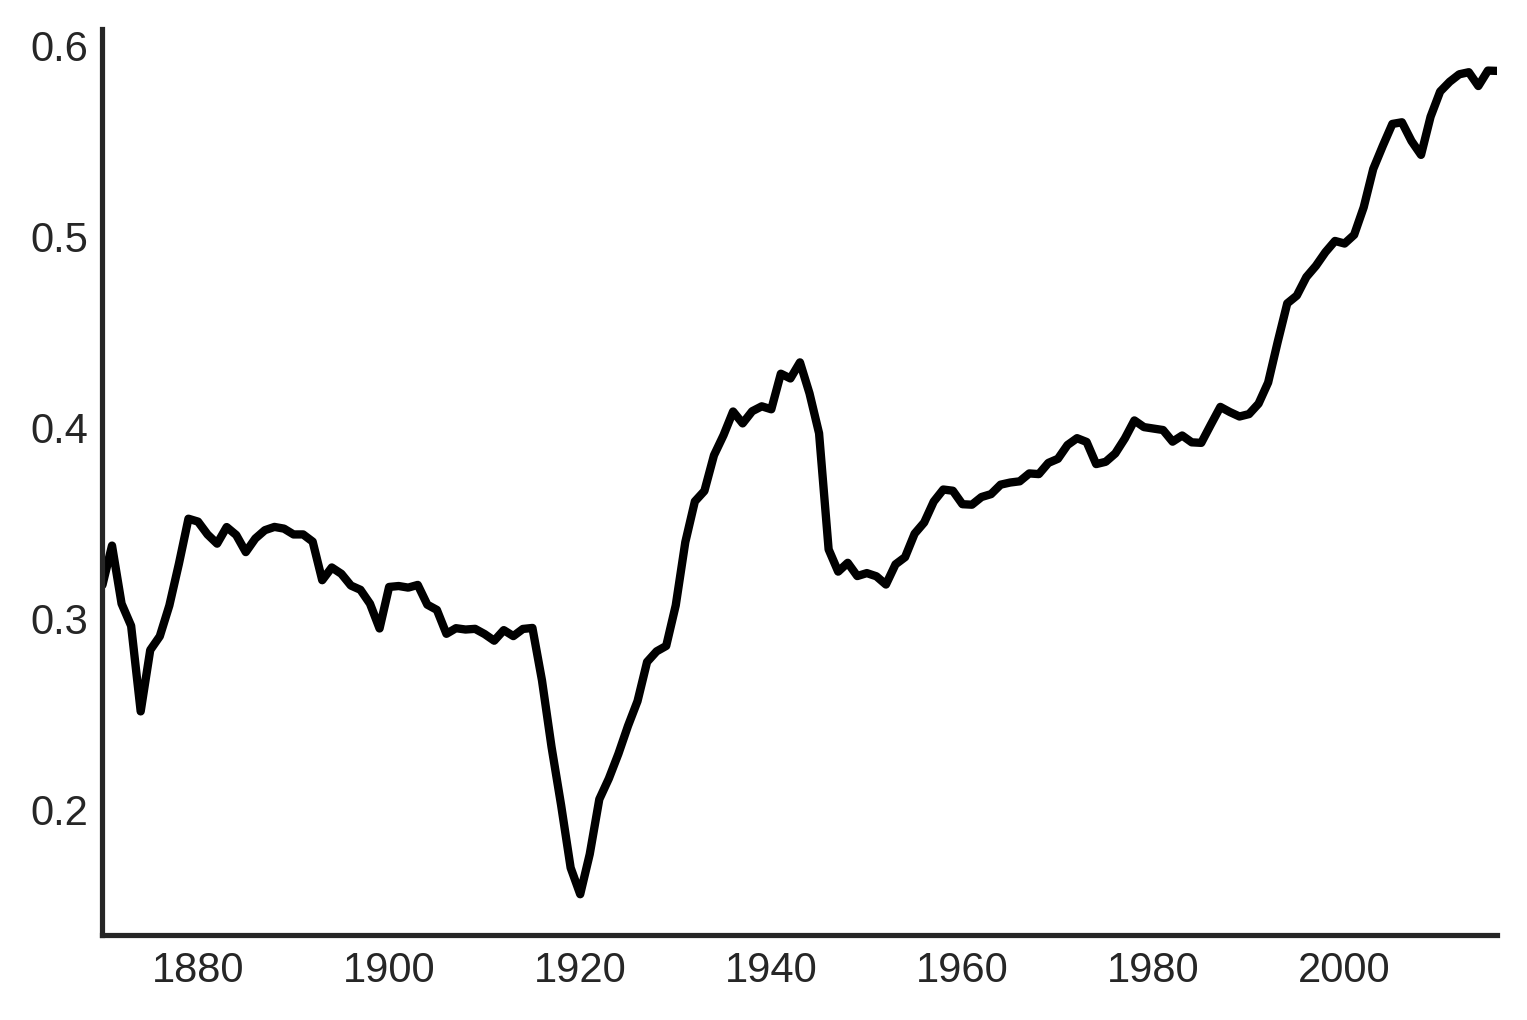
\includegraphics[width=.5\paperwidth, height=.43\paperheight]{./figs/Jorda_Mean.png}
	\caption*{\textbf{Fonte:} \textcite{jorda_rate_2019}}
\end{figure}
    
\end{frame}